\clearpage
\section{ZigBee Packet Structure }
\label{AppendixF} % For referencing this appendix elsewhere, use 

\subsection{API Frames}
\begin{figure}[htbp]
\centering
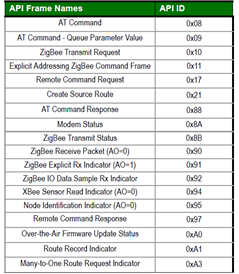
\includegraphics[height=10cm]{api3}
\caption{API Frame Names and Values ( $\circlearrowleft$ \ref{api1} )}
\label{fig:api3 }
\end{figure}
\clearpage
\pagebreak
%------------------------------------
\subsection{ZigBee Transmit Request}
\begin{figure}[htbp]
\centering
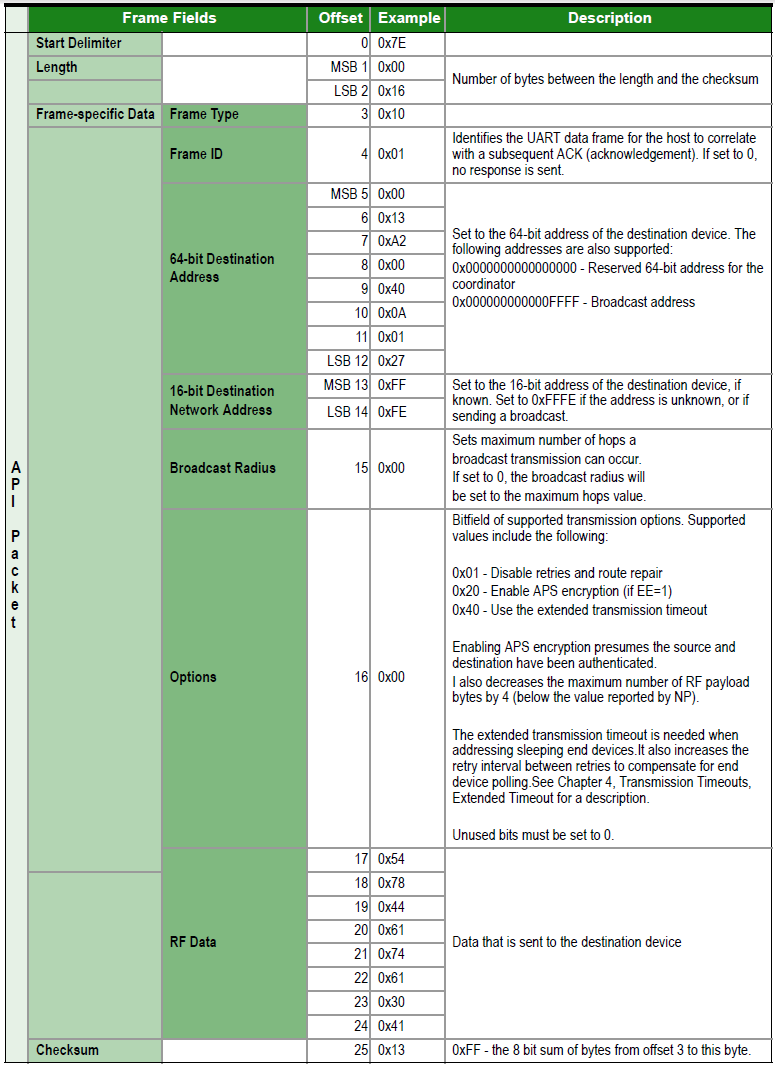
\includegraphics[height=18cm]{api4}
\caption{ZigBee Transmit Request Frame Structure ( $\circlearrowleft$ \ref{api1} )}
\label{fig:api4}
\end{figure}
\clearpage
\pagebreak
%------------------------------------
\subsection{ZigBee Receive Packet}
\begin{figure}[htbp]
\centering
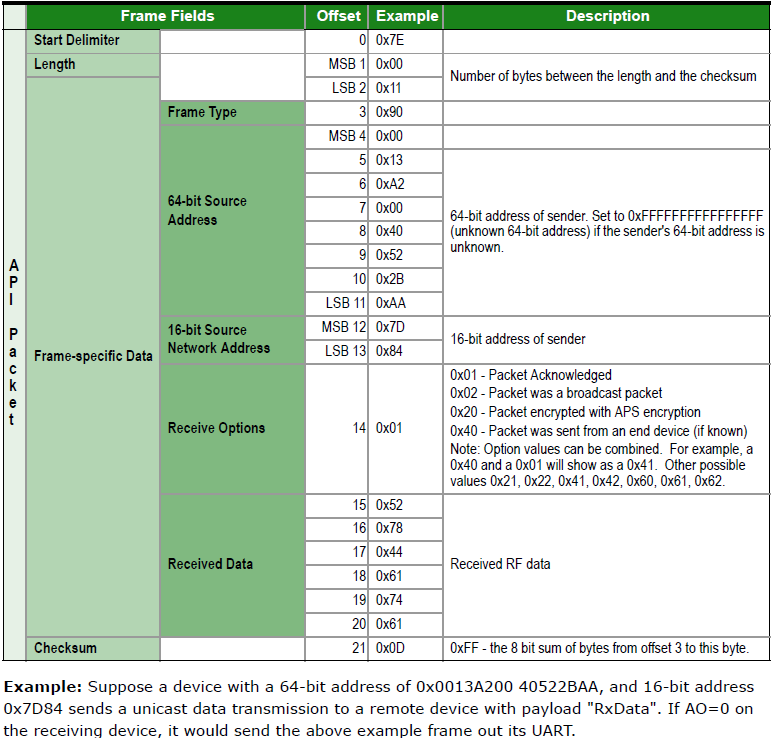
\includegraphics[height=16cm]{api5}
\caption{ZigBee Receive Packet Frame Structure ( $\circlearrowleft$ \ref{api1} )}
\label{fig:api5}
\end{figure}
\clearpage
\pagebreak
%------------------------------------
\subsection{Waspmote Application Header in ZigBee API Frame Structure}
\begin{figure}[htbp]
\centering
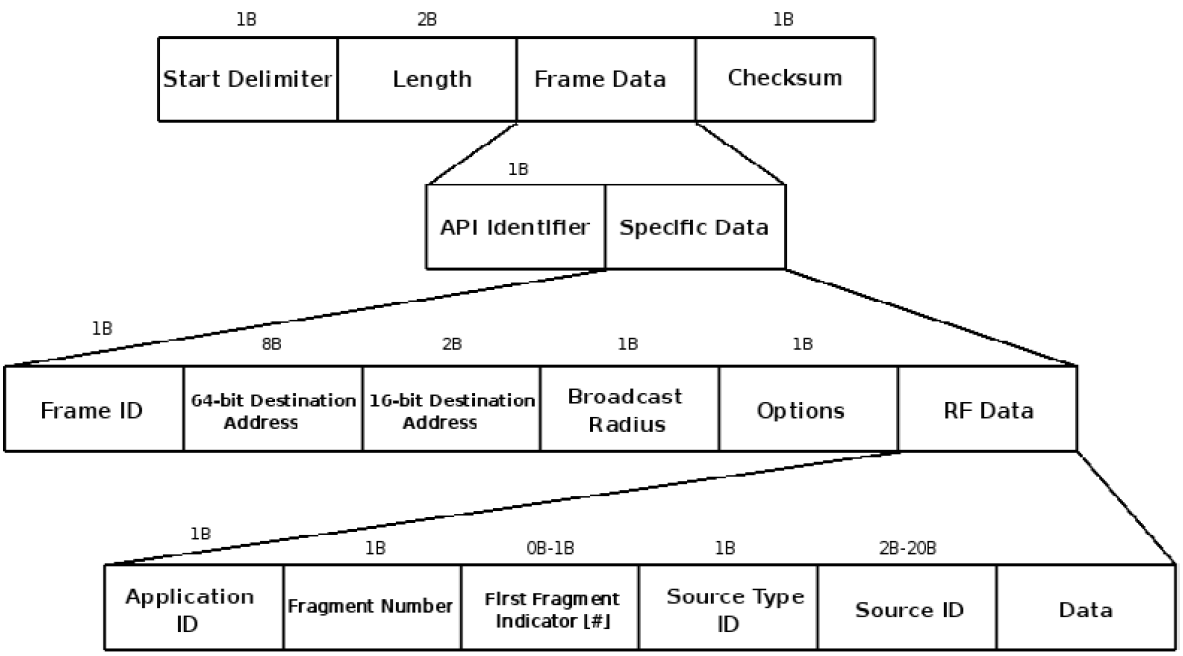
\includegraphics[height=10cm]{frames}
\caption{Waspmote Application Header in ZigBee API Frame Structure ( $\circlearrowleft$  \ref{frames1}    $ \hspace{0.2cm}\circlearrowleft$ \ref{ZBStructure} )}
\label{fig:frames}
\end{figure}
\clearpage
\pagebreak
%------------------------------------
\subsection{IO API Data Frames for Waspmote and Gateway}
\label{OwnProtocolLabel}
\begin{figure}[htbp]
\centering
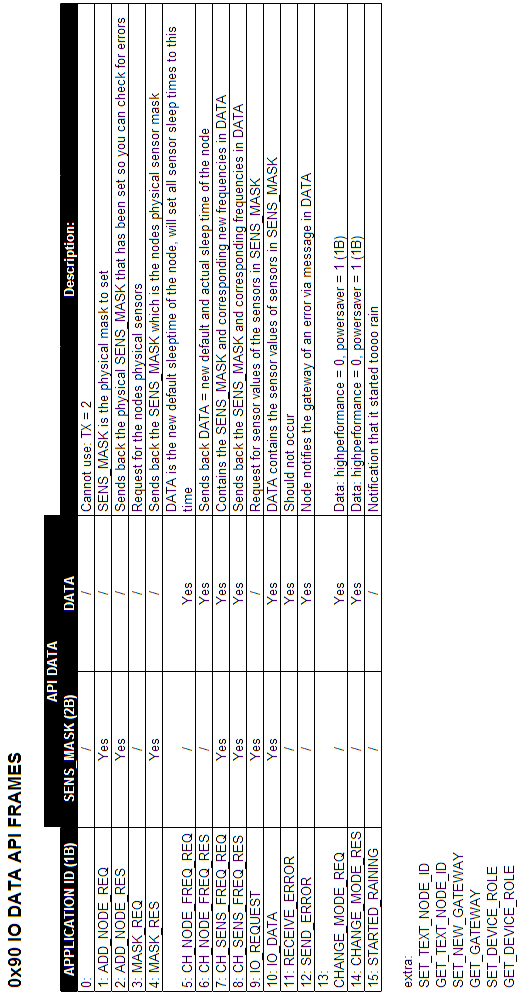
\includegraphics[height=18cm]{AppIDs}
\caption{IO API Data Frames for Waspmote and Gateway ( $\circlearrowleft$ \ref{frames1} )}
\label{fig:OwnProtocol}
\end{figure}
%------------------------------------
\clearpage
\pagebreak
\subsection{Web service packets}
\label{xml}
An XML example of the different HTTP POST request that can be made to the web service. The full url becomes: \verb+(webserviceIP)/url+\\
Url is replace by the url’s found below for each request. The web service IP is currently not fixed and has to be determined upon installation of the gateway. It is also possible that a domain name will be added. This will be something like WSN.groupt.be. The XML is sent as POST data in a HTTP request. All Each ID relates to the corresponding ID in Ipsum. The client will create installations, sensor groups and sensors in Ipsum and then send all these ID’s to the gateway so the gateway knows to which Ipsum sensor to upload data or from which sensor change frequencies.\\
\begin{figure}[htbp]
\centering
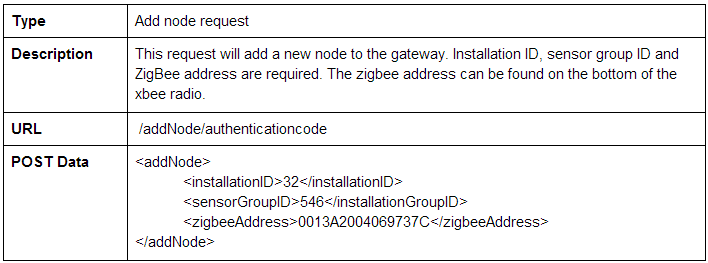
\includegraphics[width=0.98\textwidth]{add}
\caption{An Add node request}
\end{figure}

\begin{figure}[htbp]
\centering
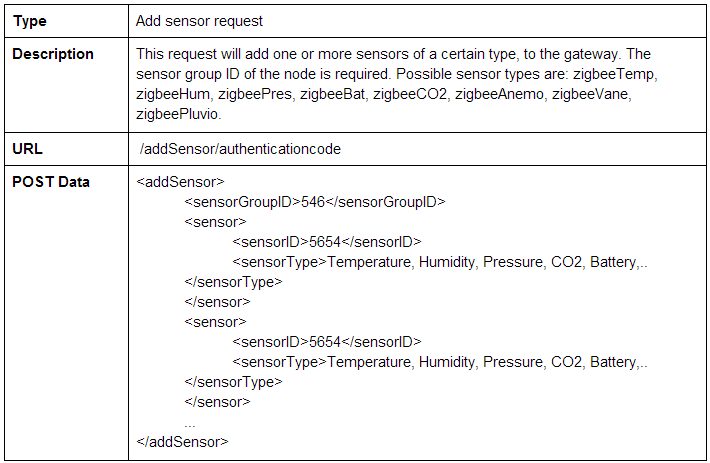
\includegraphics[width=0.98\textwidth]{addSens}
\caption{An Add sensor request}
\end{figure}

\begin{figure}[htbp]
\centering
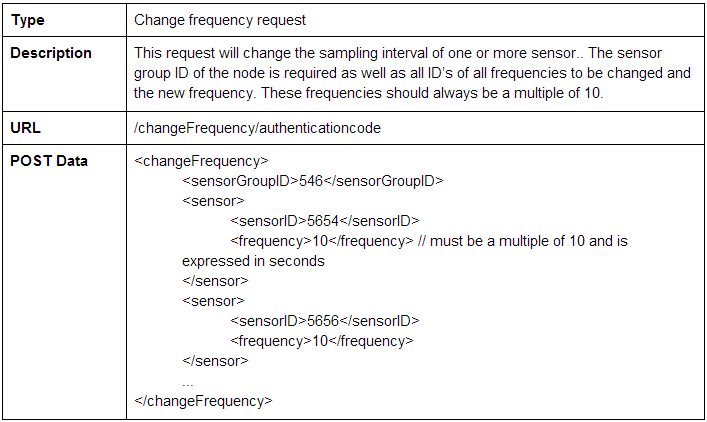
\includegraphics[width=0.98\textwidth]{change}
\caption{A change frequency request}
\end{figure}

\begin{figure}[htbp]
\centering
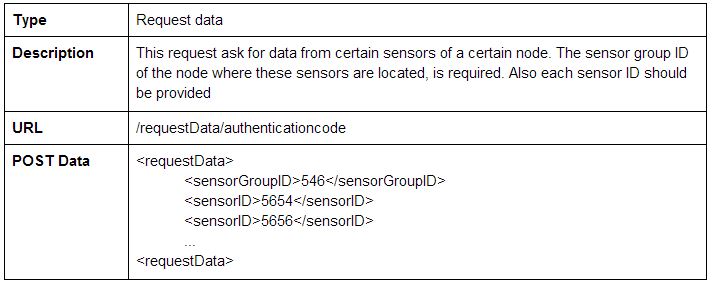
\includegraphics[width=0.98\textwidth]{change2}
\caption{A data request}
\end{figure}